This procedure by \citep{DolsekFajfar2004} provides a simple relationship between inelastic displacement of a SDoF system and the corresponding median elastic spectral displacement value. The procedure presented herein is applicable to any kind of multi-linear capacity curve and it can be used to estimate single building fragility curves. Moreover the fragility curves derived for single buildings can be combined into a unique fragility curve, which considers also the inter-building uncertainty.\\

The relationship provided by \citep{DolsekFajfar2004} has been adapted for MDoF systems, relating the inelastic top displacement of a structure $\hat{d}_{roof}$ to the median elastic spectral acceleration value at its fundamental period of vibration $\hat{S}_{a}(T_1)$, as presented in the following equation:

\begin{equation}
\hat{S}_a(T_1) = \frac{4 \pi^2}{\hat{C}_R T^2 \Gamma_1 \Phi_1} \hat{d}_{roof}
\label{eq:basic_DF}
\end{equation}

where $\Gamma_1 \Phi_1$ is the first mode participation factor estimated for the first-mode shape normalised by the roof displacement. The value of C$_R$, the ratio between the inelastic and the elastic spectral displacement, is found from the following equation:

\begin{equation}
\hat{C}_{R} = \frac{\mu}{R(\mu)}
\label{eq:Cr_DF}
\end{equation}

where $\mu$ and $R$ are the median values of ductility level and the reduction factor for that level of ductility respectively. R is defined as the ratio between the spectral acceleration S$_a$ and the yielding capacity of the system S$_{ay}$.  According to the results of an extensive parametric study using three different sets of recorded and semi-artificial ground motions, \citep{DolsekFajfar2004} related the ductility demand $\mu$ and reduction factor R through the following formula:

\begin{equation}
\label{eq:mu_DF}
\mu = \frac{1}{c} (R-R_{0})+\mu_{0}
\end{equation}

In the proposed model $\mu$ is linearly dependent on R within two reduction factor intervals. The parameter c defines the slope of the R–$\mu$ relation, and it depends on the idealised pushover curve parameters (the initial period of the system T, the maximum to residual strength ratio r$_{u}$, the ductility at the onset of degradation $\mu_s$) and the corner periods T$_{c}$ and T$_{d}$. T$_{c}$ and T$_{d}$ are the corner periods between the constant acceleration and constant velocity part of the idealised elastic spectrum, and between the constant velocity and constant displacement part of the idealised elastic spectrum respectively. $R_{0}$ and $\mu_{0}$ are the values of R and $\mu$ on the capacity curve corresponding to the onset of hardening or softening behaviour, according to the following relationship:

\begin{equation}
\mu_0= 1 ... if R<=R(\mu_s); \mu_0 = \mu_s ... if R>R(\mu_s)
\end{equation}
\begin{equation}
R_0= 1 ... if R<=R(\mu_s); R_0 = R(\mu_s) ... if R>R(\mu_s)
\end{equation}

Given the parameters of the multi-linear pushover curves (R$_{0}$, $\mu_{0}$, r$_{u}$, $\mu_s$) and T, the median R-$\mu$ curve can be constructed using the aforementioned relationship, as presented in the following Figure.

\begin{figure}[!htbp]
\centering
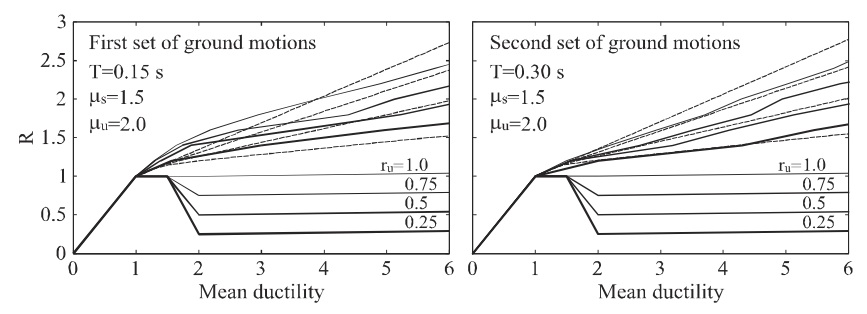
\includegraphics[width=15cm]{figures/DF_R-mu.jpg}
\caption{R-$\mu$ curves derived from Pushover curve.}
\end{figure}

The relationship between the 16$^{th}$ and 84$^{th}$ fractiles of $\mu$ and R$_{50}$ needs to be derived using the equations from \citep{RuizGarciaMiranda2007} instead, given that \citep{DolsekFajfar2004} do not provide estimates of the dispersion of R. This is done by computing the value of record-to-record dispersion in terms of top displacement $\beta_{\theta d}$ for a number of R with Equation~\ref{eq:beta_eq_RGM}, and calculating the 16$^{th}$ and 84$^{th}$ fractiles of $\mu$ ($\mu_{16\%}$ and $\mu_{84\%}$), according to the Equations \ref{eq:mu16-beta} and \ref{eq:mu84-beta}. The $\mu_{50\%}-R_{50\%}$, $\mu_{16\%}-R_{50\%}$ and $\mu_{84\%}-R_{50\%}$ curves can thus be drawn, as shown in Figure \ref{fig:R-mu}.

\begin{figure}[!htbp]
\centering
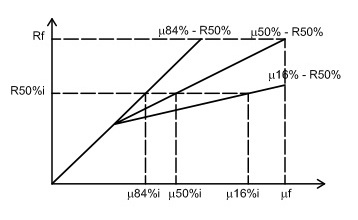
\includegraphics[width=8cm]{figures/Rmu.jpg}
\caption{$\mu_{50\%}-R_{50\%}$, $\mu_{16\%}-R_{50\%}$ and $\mu_{84\%}-R_{50\%}$ curves}
\label{fig:R-mu}
\end{figure}

\begin{equation}
\mu_{ds,16} = \hat{\mu}_{ds} e^{-\beta_{\theta d,ds}}
\label{eq:mu16-beta}
\end{equation}
\begin{equation}
\mu_{ds,84} = \hat{\mu}_{ds} e^{\beta_{\theta d,ds}}
\label{eq:mu84-beta}
\end{equation}

For any inelastic displacement, and therefore any level of ductility $\mu$, the corresponding $R_{50\%}$, $R_{16\%}$, and $R_{84\%}$ values are found by interpolating the aforementioned curves. Median $R$ and its dispersion at ductility levels corresponding to the damage thresholds ds can thus be determined, and converted into median $S_{a, ds}$ and its dispersion due to record-to-record variability $\beta_{S_{a d}}$ according to equations \ref{eq:SaR} and \ref{eq:betaR}. \\

If dispersion in the damage state threshold is different from zero, different values of ductility limit state are sampled from the lognormal distribution with the median value of the ductility limit state, and dispersion of the input $\beta_{\theta c}$. For each of these ductilities the corresponding $R_{50\%}$, $R_{16\%}$, and $R_{84\%}$ values are found by interpolating the $\mu_{50\%}-R_{50\%}$, $\mu_{16\%}-R_50\%$ and $\mu_{84\%}-R_50\%$ curves, and converting into $\hat{S}_{a,ds}$ and $\beta_{S_{a d}}$ according to Equations \ref{eq:SaR} and \ref{eq:betaR}. Monte Carlo random S$_a$ for each of the sampled ductility limit states are computed using $\hat{S}_{a,ds}$ and $\beta_{S_{a d}}$, and their median and dispersion are estimated. These parameters constitute the median $\hat{S}_{a,ds}$ and the total dispersion $\beta_{S_a}$ for the considered damage state. The procedure is repeated for each damage state.\\

If multiple buildings have been input to derive fragility function for a class of buildings, all $\hat{S}_{a, blg}$ and $\beta_{S_a, blg}$ are combined into a single lognormal curve as described in section \ref{subsec:SPO2IDA}. \\

In order to use this methodology, it is necessary to load one or multiple capacity curves as described in Section \ref{subsec:cap_curves}. The pushover curve input type needs to be either Base Shear vs Roof Displacement (Section \ref{subsubsec:VB-Droof}), or Base Shear vs Floor Displacements (Section \ref{subsubsec:VB-Dfloor}). The capacity curves are then idealised with a bilinear elasto-plastic shape. It is also necessary to specify the type of shape the capacity curves should be idealised with, using the parameter \verb=idealised_type= (either \verb=bilinear= or \verb=quadrilinear=). If the user has already an idealised multilinear pushover curve for each building, the variable \verb=Idealised= in the csv input file should be set to \verb=TRUE=, and idealised curves should be provided according to section \ref{subsec:cap_curves}. Then, it is necessary to specify a damage model using the parameter \verb=damage_model= (see Section \ref{subsec:dmg_model}). The inter-storey drift based damage model described in \ref{subsubsec:isd-dmg} should be used for this method.

If dispersion due to uncertainty in the limit state definition is different from zero, a Monte Carlo sampling needs to be performed to combine it with the record-to-record dispersion. The number of Monte Carlo samples should be defined in the variable \verb=montecarlo_samples=.
After importing the module DF2004, it is possible to calculate the parameters of the fragility model, median and dispersion, using the following command:

\begin{Verbatim}[frame=single, commandchars=\\\{\}, samepage=true]
fragility_model = DF2004.calculate_fragility(capacity_curves, ...
idealised_capacity, damage_model, montecarlo_samples, Sa_ratios, ...
corner_periods)
\end{Verbatim}

where \verb=Sa_ratios= is a variable needed to combine together fragility curves for many buildings, as described in Section \ref{subsec:SPO2IDA}.